%iffalse
\let\negmedspace\undefined
\let\negthickspace\undefined
\documentclass[journal,12pt,onecolumn]{IEEEtran}
\usepackage{cite}
\usepackage{amsmath,amssymb,amsfonts,amsthm}
\usepackage{algorithmic}
\usepackage{graphicx}
\usepackage{textcomp}
\usepackage{xcolor}
\usepackage{txfonts}
\usepackage{listings}
\usepackage{enumitem}
\usepackage{mathtools}
\usepackage{gensymb}
\usepackage{comment}
\usepackage[breaklinks=true]{hyperref}
\usepackage{tkz-euclide} 
\usepackage{listings}
\usepackage{gvv}                                        
%\def\inputGnumericTable{}                                 
\usepackage[latin1]{inputenc}                                
\usepackage{color}                                            
\usepackage{array}                                            
\usepackage{longtable}                                       
\usepackage{calc}                                             
\usepackage{multirow}                                         
\usepackage{hhline}                                           
\usepackage{ifthen}                                           
\usepackage{lscape}
\usepackage{tabularx}
\usepackage{array}
\usepackage{float}

\usepackage{enumitem}
\usepackage{xcolor}
%\usepackage{multicol}


\newtheorem{theorem}{Theorem}[section]
\newtheorem{problem}{Problem}
\newtheorem{proposition}{Proposition}[section]
\newtheorem{lemma}{Lemma}[section]
\newtheorem{corollary}[theorem]{Corollary}
\newtheorem{example}{Example}[section]
\newtheorem{definition}[problem]{Definition}
\newcommand{\BEQA}{\begin{eqnarray}}
\newcommand{\EEQA}{\end{eqnarray}}
\newcommand{\define}{\stackrel{\triangle}{=}}
\theoremstyle{remark}
\newtheorem{rem}{Remark}

\title{9.5.11}
\author{AI24BTECH11021 - Manvik Muthyapu}
\begin{document}
\bibliographystyle{IEEEtran}

\maketitle
\bigskip

\renewcommand{\thefigure}{\theenumi}
\renewcommand{\thetable}{\theenumi}


\textbf{Question}:\\
Prove that the curves $y^2 = 4x$ and $x^2 = 4y$ divide the area of the square bounded by sides $x=0, x=4, y=4,$ and $y=0$ into three equal parts.
\hfill{(12, 2018)}

\solution
First, to find points of intersection, substitute $x = \frac{y^2}{4}$ into $x^2 = 4y$:

\begin{align}
	\brak{\frac{y^2}{4}}^2 &= 4y \\
	\frac{y^4}{16} &= 4y \\
	\implies y^4 &= 64y \\
	\implies y(y^3 - 64) &= 0 \implies y = 0,4
\end{align}

So, the points of intersection are (0,0) and (4,4). \\
Area of the Square $= 4 \times 4 = 16$.\\ 
Area under the curve $y^2 = 4x$ between $y = 0$ and $y = 4$,

\begin{align}
	\text{Area} &= \int_0^4 \frac{y^2}{4} \, dy = \frac{1}{4} \int_0^4 y^2 \, dy \\
	&= \frac{1}{4} \sbrak{\frac{y^3}{3}}_0^4 = \frac{1}{4} \times \frac{64}{3} \\
	&= \frac{16}{3}
\end{align}

Area under the $x^2 = 4y$ between $x = 0$ and $x = 4$,

\begin{align}
	\text{Area} &= \int_0^4 \frac{x^2}{4} \, dx = \frac{1}{4} \int_0^4 x^2 \, dx \\
	&= \frac{1}{4} \sbrak{\frac{x^3}{3}}_0^4 = \frac{1}{4} \times \frac{64}{3} \\
	&= \frac{16}{3}
\end{align}

Remaining area,
$$16 - \frac{16}{3} + \frac{16}{3} = \frac{16}{3}$$

$\therefore$ The areas are equal.

\begin{figure}[h!]
	\centering
	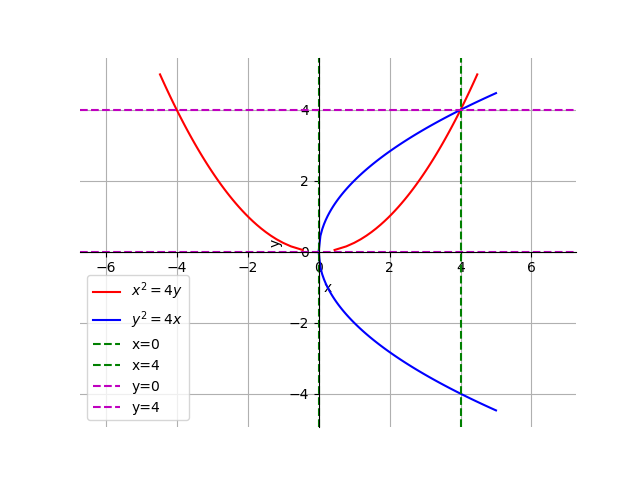
\includegraphics[width=0.7\linewidth]{figs/plot.png}
\end{figure}

\end{document}
